\documentclass[11pt]{article}
\usepackage[margin=1in]{geometry}
\usepackage{authblk}
\usepackage{amsmath,amssymb}
\usepackage{graphicx}
\usepackage{caption}
\usepackage{subcaption}
\usepackage{float}
\usepackage{placeins}
\usepackage{array}
\usepackage{booktabs}
\usepackage{tabularx}
\usepackage[numbers,sort&compress]{natbib}
\usepackage{lineno} % Line numbers for peer review
\usepackage{hyperref}
\hypersetup{colorlinks=true,linkcolor=black,citecolor=black,urlcolor=black}

\graphicspath{{figures_supp/}{figures/}}

\newcolumntype{Y}{>{\raggedright\arraybackslash}X}
\newcolumntype{C}{>{\centering\arraybackslash}X}
\captionsetup[subfigure]{labelformat=empty,skip=0pt}

% Supplementary numbering (S1, S2, ...; Figure S1; Table S1)
\renewcommand{\thesection}{S\arabic{section}}
\renewcommand{\thesubsection}{S\arabic{section}.\arabic{subsection}}
\renewcommand{\thesubsubsection}{S\arabic{section}.\arabic{subsection}.\arabic{subsubsection}}
\renewcommand{\thefigure}{S\arabic{figure}}
\renewcommand{\thetable}{S\arabic{table}}

\begin{document}
\linenumbers % Enable line numbers for peer review

% Custom title for double-blind review
\begin{center}
{\LARGE\bfseries Supplementary Materials for:\\
Competing feedback channels drive phase transitions in collective~emotion}
\end{center}

\vspace{1em}

\renewcommand{\contentsname}{Supplementary Contents}
\setcounter{tocdepth}{2}
\tableofcontents
\clearpage
\FloatBarrier

\section*{Guide to this Supplementary Materials}
\addcontentsline{toc}{section}{Guide to this Supplementary Materials}
Core results are reported in the main text; this supplement provides supporting methodological details and auxiliary analyses. Sections S1--S2 expand the \emph{Materials and Methods}, and Sections S3--S6 provide supporting figures referenced from the \emph{Results}. The main text cites these materials as ``Supplementary Materials S\#'' and ``Supplementary Fig.~S\#''.

\noindent\textbf{Contents overview.}
\begin{itemize}
  \item \textbf{Supplementary Methods}
  \begin{itemize}
    \item \textbf{S1} LLM annotation protocol and validation.
    \item \textbf{S2} Mean-field derivations for the critical point and Ginzburg--Landau form.
  \end{itemize}
  \item \textbf{Supplementary Results}
  \begin{itemize}
    \item \textbf{S3} Network validation details and order-parameter conventions.
    \item \textbf{S4} Early-warning signal analysis for critical slowing down.
    \item \textbf{S5} Parameter effects on the critical boundary.
    \item \textbf{S6} Empirical analysis details and density diagnostics.
  \end{itemize}
\end{itemize}
\vspace{0.4em}
\noindent\textbf{Quick reference (main text $\leftrightarrow$ supplement).}
\begin{center}
  \footnotesize
  \begin{tabular}{@{}ll@{}}
    \toprule
    Main text & Supplementary location \\
    \midrule
    Methods: LLM annotation & S1 \\
    Methods: mean-field derivations & S2 \\
    Results: direction--intensity coupling & Fig.~\ref{fig:supp:tau-ratio} (S3) \\
    Results: robustness across networks & Figs.~\ref{fig:supp:signed-vs-abs-q}--\ref{fig:supp:susceptibility-fss} (S3) \\
    Results: critical slowing down & Figs.~\ref{fig:supp:ews-ac-var}--\ref{fig:supp:abm-multilag-ac} (S4) \\
    Results: parameter landscape & Figs.~\ref{fig:supp:symmetric-diagonal}--\ref{fig:supp:param-importance} (S5) \\
    Results: empirical signatures & Figs.~\ref{fig:supp:time-series-overview}--\ref{fig:supp:h2-density-12h} (S6) \\
    \bottomrule
  \end{tabular}
\end{center}

\noindent\textbf{Notation.}
Supplementary Table~\ref{tab:supp:notation} summarizes the main symbols used throughout the paper, together with baseline values and ranges where applicable.
\begin{table}[H]
  \centering
  \caption{Notation and baseline values.}
  \label{tab:supp:notation}
  \footnotesize
  \begin{tabularx}{\textwidth}{@{}lYY@{}}
    \toprule
    Symbol & Meaning & Baseline / definition \\
    \midrule
    \multicolumn{3}{@{}l}{\textbf{Model state and environment}} \\
    \addlinespace[0.2em]
    $H,M,L$ & high/medium/low arousal states & --- \\
    $\rho_H,\rho_M,\rho_L$ & population fractions in $H,M,L$ & --- \\
    $q$ & polarization direction ($q=\rho_H-\rho_L$) & $q\in[-1,1]$ \\
    $a$ & activity / moderate-buffer depletion ($a=\rho_H+\rho_L=1-\rho_M$) & $a\in[0,1]$; in data $a=X_H+X_L$ \\
    $Q$ & observed polarization order parameter & ABM: analog of $q$; data: $Q=X_H-X_L$ \\
    $p_{\text{env}}$ & perceived risk probability in the mixed environment & weighted mixture of channel risks (Section~S2) \\
    \addlinespace[0.35em]
    \multicolumn{3}{@{}l}{\textbf{Model parameters}} \\
    \addlinespace[0.2em]
    $\phi$ & high-arousal threshold & 0.54 \\
    $\theta$ & low-arousal threshold & 0.46 \\
    $k$ & signals sampled per update (information density) & 50 (baseline); scanned 10--500 \\
    $n_m$ & mainstream channel strength & 10 \\
    $n_w$ & user-generated channel strength & 5 \\
    $n_w/n_m$ & media ratio (user-generated vs.\ mainstream strength) & 0.5 (baseline); scanned 0.2--2.0 \\
    $r$ & channel-balance control parameter & varied in $[0,1]$ \\
    $\beta$ & local coupling strength (ABM) & 0 (baseline); varied up to 0.2 \\
    \addlinespace[0.35em]
    \multicolumn{3}{@{}l}{\textbf{Simulation settings and diagnostics}} \\
    \addlinespace[0.2em]
    $N$ & population size & varies by figure \\
    $\langle k\rangle$ & network average degree & 50 (unless stated otherwise) \\
    $f$ & update fraction per step & 0.1; 1 sweep $=N$ updates $=1/f$ steps \\
    $U_4(r;N)$ & Binder cumulant used for finite-size scaling & $1-\langle Q^4\rangle/(3\langle Q^2\rangle^2)$ \\
    \addlinespace[0.35em]
    \multicolumn{3}{@{}l}{\textbf{Theory quantities}} \\
    \addlinespace[0.2em]
    $\chi$ & psychological sensitivity of collective response & $\chi=\left.\frac{d\mathcal{S}}{dp}\right|_{p=1/2}$ \\
    $\Gamma(r)$ & feedback gradient of $p_{\text{env}}$ around $q=0$ & defined in Section~S2 \\
    $r_c$ & critical point (stability boundary) & defined in Section~S2 \\
    $\Delta r_c$ & ABM--theory deviation in the estimated boundary & $\Delta r_c=r_c^{\mathrm{ABM}}-r_c^{\mathrm{theory}}$ \\
    $\tau$ & relaxation time near criticality & $\tau\sim 1/|r_c-r|$ as $r\to r_c^-$ \\
    $\tau_a/\tau_q$ & relaxation-time ratio (activity vs.\ polarization) & estimated in asymmetric simulations; $\approx 0.70$ (Fig.~\ref{fig:supp:tau-ratio}) \\
    $\mathrm{AC}_1$ & lag-1 autocorrelation & computed from steady-state $Q(t)$ \\
    \addlinespace[0.35em]
    \multicolumn{3}{@{}l}{\textbf{Empirical proxies}} \\
    \addlinespace[0.2em]
    $X_H,X_M,X_L$ & fractions of posts labeled $H/M/L$ within a time window & --- \\
    $r_{\text{proxy}}$ & user-generated dominance proxy &
    $n_{\text{wemedia}}/(n_{\text{wemedia}}+n_{\text{mainstream}}+n_{\text{government}})$ \\
    $\sigma_Q$ & volatility within a segment & $\sigma_Q=\mathrm{std}(Q)$ \\
    $\text{jump}_{q95}$ & jump intensity within a segment & 95th percentile of $|\Delta Q/\Delta t|$ \\
    \bottomrule
  \end{tabularx}
\end{table}
\FloatBarrier

\section*{Supplementary Methods}
\addcontentsline{toc}{section}{Supplementary Methods}
\noindent Sections S1--S2 provide additional methodological details for the empirical annotation pipeline and the mean-field derivations.
\FloatBarrier

% -------------------------
% S1: LLM annotation protocol
% -------------------------
\section{LLM annotation protocol}
\label{supp:s1-llm}

We annotate Weibo posts along two dimensions---emotional arousal and risk content---using \texttt{Qwen/Qwen3-8B} \citep{Qwen3_8B}. Prompts are structured and enforce a fixed JSON output schema to improve reproducibility.

\subsection{Annotation setup}
We serve the model via a local OpenAI-compatible API. Inference uses temperature $=0.1$ and max\_tokens $=512$.

\subsection{Label definitions}
\noindent\textbf{Emotional arousal (\texttt{emotion\_class}).}
\begin{itemize}
  \item \textbf{H}: strong emotional activation (anger, panic/fear, sarcasm/insults, highly emotional accusations).
  \item \textbf{M}: neutral or informational content (calm discussion, explanations, supportive messages).
  \item \textbf{L}: negative but low-intensity emotions (worry, confusion, helplessness, sadness).
\end{itemize}

\noindent\textbf{Risk content (\texttt{risk\_class}).}
\begin{itemize}
  \item \textbf{risk}: conveys negative health impacts of COVID-19/long COVID (symptoms, severity, sequelae, warnings).
  \item \textbf{norisk}: emphasizes recovery/controllability or reassurance, criticizes fear-mongering, or is unrelated to health risks.
\end{itemize}

\subsection{Prompt structure and JSON output}
The prompt specifies the above criteria, forbids any free-form text beyond a single JSON object, and requests confidence scores in $[0,1]$. Output fields are:
\texttt{emotion\_class}, \texttt{emotion\_confidence}, \texttt{risk\_class}, \texttt{risk\_confidence}, and a brief \texttt{reasoning} string.

\subsection{Prompt template (English translation)}
\label{supp:s1-prompt-template}
The annotation prompt is implemented as a system message containing the task definitions and criteria, followed by a user message containing the post text. For readability, we show an English translation of the core prompt template below (the original Chinese prompt is provided in the code repository).
\begin{verbatim}
[System]
You are a social-media content analyst. Classify the following Weibo post along:
1) emotional arousal (H/M/L) and 2) health-risk content (risk/norisk).
Return ONLY a single JSON object. No markdown, no extra text.

Output fields (JSON):
  emotion_class: "H" | "M" | "L"
  emotion_confidence: float in [0,1]
  risk_class: "risk" | "norisk"
  risk_confidence: float in [0,1]
  reasoning: <= 20 words

Emotion (emotion_class):
  H: strong emotion (anger, panic/fear, sarcasm/insults, emotional accusations)
  M: neutral/informational (calm discussion, explanations, supportive messages)
  L: negative but low-intensity (worry, confusion, helplessness, sadness)

Risk (risk_class):
  risk: conveys negative health impacts of COVID-19/long COVID (symptoms, warnings)
  norisk: reassurance/recovery/controllability, critiques fear-mongering, or unrelated

If the post is too short or contains only hashtags with no substantive content:
  default emotion_class=M and risk_class=norisk with confidence=0.5.

[User]
Post: {post_text}

[Output]
Return ONLY a valid JSON object matching the schema below.
\end{verbatim}

\subsection{JSON schema}
\label{supp:s1-json-schema}
The model output is constrained to a fixed JSON object with the following fields:
\begin{verbatim}
{
  "emotion_class": "H" | "M" | "L",
  "emotion_confidence": 0.0 - 1.0,
  "risk_class": "risk" | "norisk",
  "risk_confidence": 0.0 - 1.0,
  "reasoning": "<=20 words>"
}
\end{verbatim}
We discard any response that does not parse as JSON or violates the allowed label set.

\subsection{Validation}
We compared LLM-assigned labels to manual ratings on a validation subset ($n=5{,}000$) randomly sampled from the corpus after de-duplication by post identifier (\texttt{mid}). To reduce anchoring effects, manual labels were collected in a blind annotation sheet that does not include LLM outputs, and the LLM labels were joined only at scoring time. Exact-match accuracy was 85\% for arousal labels (Cohen's $\kappa=0.79$) and 87\% for risk labels ($\kappa=0.82$). Fine-grained metrics and confusion matrices are reported in Supplementary Tables~\ref{tab:supp:llm-emotion-metrics}--\ref{tab:supp:llm-risk-confusion}.

\subsection{Fine-grained performance metrics}
\label{supp:s1-fine-grained-metrics}
For each class, we compute precision and recall from the confusion matrix and report 95\% confidence intervals using Wilson score intervals. F1-score intervals are obtained by propagating the corresponding precision/recall bounds through $F_1=2PR/(P+R)$.
\begin{table}[H]
  \centering
  \caption{Fine-grained performance metrics for three-class emotional arousal classification (H/M/L; $n=5{,}000$).}
  \label{tab:supp:llm-emotion-metrics}
  \footnotesize
  \begin{tabular}{@{}lccc@{}}
    \toprule
    Category & Precision [95\% CI] & Recall [95\% CI] & F1-score [95\% CI] \\
    \midrule
    H (high arousal) & 0.86 [0.84, 0.88] & 0.84 [0.82, 0.86] & 0.85 [0.83, 0.87] \\
    M (medium arousal) & 0.83 [0.81, 0.85] & 0.87 [0.85, 0.89] & 0.85 [0.83, 0.87] \\
    L (low arousal) & 0.86 [0.84, 0.88] & 0.84 [0.82, 0.86] & 0.85 [0.83, 0.87] \\
    \midrule
    Overall & \multicolumn{3}{l}{Accuracy = 0.85, Cohen's $\kappa$ = 0.79} \\
    \bottomrule
  \end{tabular}
\end{table}

\begin{table}[H]
  \centering
  \caption{Confusion matrix for emotional arousal classification (H/M/L; $n=5{,}000$).}
  \label{tab:supp:llm-emotion-confusion}
  \footnotesize
  \begin{tabular}{@{}lccc@{}}
    \toprule
    & \multicolumn{3}{c}{Predicted} \\
    \cmidrule(l){2-4}
    Actual & H & M & L \\
    \midrule
    H & \textbf{1412} & 185 & 83 \\
    M & 124 & \textbf{1451} & 95 \\
    L & 106 & 112 & \textbf{1432} \\
    \bottomrule
  \end{tabular}
\end{table}

\begin{table}[H]
  \centering
  \caption{Fine-grained performance metrics for risk-content classification (\texttt{risk}/\texttt{norisk}; $n=5{,}000$).}
  \label{tab:supp:llm-risk-metrics}
  \footnotesize
  \begin{tabular}{@{}lccc@{}}
    \toprule
    Category & Precision [95\% CI] & Recall [95\% CI] & F1-score [95\% CI] \\
    \midrule
    \texttt{norisk} & 0.89 [0.88, 0.90] & 0.92 [0.91, 0.93] & 0.90 [0.89, 0.91] \\
    \texttt{risk} & 0.81 [0.79, 0.83] & 0.75 [0.73, 0.77] & 0.78 [0.76, 0.80] \\
    \midrule
    Overall & \multicolumn{3}{l}{Accuracy = 0.87, Cohen's $\kappa$ = 0.82} \\
    \bottomrule
  \end{tabular}
\end{table}

\begin{table}[H]
  \centering
  \caption{Confusion matrix for risk-content classification (\texttt{risk}/\texttt{norisk}; $n=5{,}000$).}
  \label{tab:supp:llm-risk-confusion}
  \footnotesize
  \begin{tabular}{@{}lcc@{}}
    \toprule
    & \multicolumn{2}{c}{Predicted} \\
    \cmidrule(l){2-3}
    Actual & \texttt{norisk} & \texttt{risk} \\
    \midrule
    \texttt{norisk} & \textbf{3220} & 280 \\
    \texttt{risk} & 370 & \textbf{1130} \\
    \bottomrule
  \end{tabular}
\end{table}

% -------------------------
% S2: Mean-field derivations
% -------------------------
\section{Mean-field derivations}
\label{supp:s2-mean-field}

This note provides the derivations omitted from the main text for the mean-field critical point and the Ginzburg--Landau form.
\noindent Notation and baseline values are summarized in Supplementary Table~\ref{tab:supp:notation}.

\subsection{Mean-field update and collective response}

Under well-mixed assumptions, each update samples $k$ independent risk signals from the environment, each labeled ``risk'' with probability $p_{\text{env}}$. Let $S\sim\text{Binomial}(k,p_{\text{env}})$ and $\hat{p}=S/k$ be the perceived risk fraction. Given thresholds $\theta<\phi$, an updated individual moves to $H$ if $\hat{p}\ge \phi$, to $L$ if $\hat{p}\le \theta$, and otherwise remains in $M$. Therefore,
\begin{align}
P_H(p_{\text{env}}) &= \Pr(\hat{p}\ge \phi)=\sum_{s=\lceil k\phi\rceil}^{k}\binom{k}{s}p_{\text{env}}^{\,s}(1-p_{\text{env}})^{k-s},\\
P_L(p_{\text{env}}) &= \Pr(\hat{p}\le \theta)=\sum_{s=0}^{\lfloor k\theta\rfloor}\binom{k}{s}p_{\text{env}}^{\,s}(1-p_{\text{env}})^{k-s}.
\end{align}
The expected polarization direction after an update is the difference between high- and low-arousal outcomes,
\begin{equation}
\mathcal{S}(p_{\text{env}})=P_H(p_{\text{env}})-P_L(p_{\text{env}}).
\end{equation}
With asynchronous updates and a continuous-time approximation, the mean-field dynamics take the form
\begin{equation}
\frac{dq}{dt}=-q+\mathcal{S}(p_{\text{env}}),
\end{equation}
which is the mean-field form used in the main text.

\subsection{Linear stability and analytic critical point}

In the symmetric regime,
\begin{equation}
p^{\text{main}}(q)=\frac{1-q}{2},\qquad p^{\text{we}}(q)=\frac{1+q}{2}.
\end{equation}
The environmental risk is the weighted average of the two channels,
\begin{equation}
p_{\text{env}}(q;r)=\frac{(1-r)n_m p^{\text{main}}(q)+r n_w p^{\text{we}}(q)}{(1-r)n_m+r n_w},
\end{equation}
where $n_m$ and $n_w$ are baseline channel strengths and $r\in[0,1]$ controls their relative weight. Expanding around $q=0$ yields
\begin{equation}
p_{\text{env}}(q;r)=\frac{1}{2}+\Gamma(r)\,q+O(q^3),
\end{equation}
where the feedback gradient is
\begin{equation}
\Gamma(r)=\left.\frac{\partial p_{\text{env}}}{\partial q}\right|_{q=0}
=\frac{r n_w-(1-r)n_m}{2\left((1-r)n_m+r n_w\right)}.
\end{equation}
Next, expand the collective response around neutrality $p=1/2$:
\begin{equation}
\mathcal{S}(p)=\mathcal{S}(1/2)+\chi\left(p-\frac{1}{2}\right)+O\!\left(\left(p-\frac{1}{2}\right)^3\right),\qquad
\chi=\left.\frac{d\mathcal{S}}{dp}\right|_{p=1/2}.
\end{equation}
Under symmetry, $\mathcal{S}(1/2)=0$, so substituting $p_{\text{env}}(q;r)$ into the mean-field dynamics gives, to leading order,
\begin{equation}
\frac{dq}{dt}=(-1+\chi\Gamma)\,q+O(q^3).
\end{equation}
Therefore the neutral fixed point $q=0$ loses stability when the linear restoring coefficient changes sign:
\begin{equation}
\chi\Gamma(r_c)=1.
\end{equation}
Solving for $r$ yields the closed-form critical point reported in the main text:
\begin{equation}
r_c=\frac{n_m(\chi+2)}{n_m(\chi+2)+n_w(\chi-2)}.
\end{equation}
When $\chi\le 2$, the denominator does not admit a critical point in $[0,1]$, consistent with the absence of a transition for weak psychological sensitivity.

\subsection{Ginzburg--Landau form and noise term}

Keeping the next nonlinearity in the expansion yields a cubic term. Writing
\begin{equation}
\mathcal{S}(p)=\chi\left(p-\frac{1}{2}\right)+\frac{\mathcal{S}^{(3)}(1/2)}{6}\left(p-\frac{1}{2}\right)^3+O\!\left(\left(p-\frac{1}{2}\right)^5\right),
\end{equation}
and using $p_{\text{env}}-1/2\approx \Gamma q$, we obtain
\begin{equation}
\frac{dq}{dt}=(-1+\chi\Gamma)\,q+\frac{\mathcal{S}^{(3)}(1/2)}{6}\Gamma^3 q^3+\eta(t)+\cdots
=-\alpha q-u q^3+\eta(t)+\cdots,
\end{equation}
where $\alpha=1-\chi\Gamma$ and $u=-\mathcal{S}^{(3)}(1/2)\Gamma^3/6$. For the parameter ranges considered, $u>0$, so the dynamics can be written in the effective-potential form
\begin{equation}
\frac{dq}{dt}=-\frac{\partial V_{\text{eff}}(q)}{\partial q}+\eta(t),\qquad
V_{\text{eff}}(q)=\frac{1}{2}\alpha q^2+\frac{u}{4}q^4,
\end{equation}
which gives a pitchfork bifurcation when $\alpha$ changes sign.

The noise term $\eta(t)$ represents stochastic fluctuations induced by finite population size and discrete updates. In the large-$N$ limit, these fluctuations can be approximated as Gaussian white noise with an amplitude that scales as $1/\sqrt{N}$, implying a variance scaling as $1/N$.
\FloatBarrier

\section*{Supplementary Results}
\addcontentsline{toc}{section}{Supplementary Results}
\noindent Sections S3--S6 provide supporting figures and auxiliary analyses that complement the main-text Results and document conventions used throughout.
\FloatBarrier

% -------------------------
% S3: Network validation details
% -------------------------
\section{Network validation details and order-parameter conventions}
\label{supp:s3-theory-network}

This section clarifies the order-parameter conventions used to visualize the transition, reports the activity--polarization relaxation-time comparison under asymmetry, and documents finite-size diagnostics used to locate the transition in sparse networks.

\subsection{Order parameter under symmetric branch selection}
In the symmetric regime, different realizations can select either the $+q^\ast$ or $-q^\ast$ branch with approximately equal probability. As a result, the signed mean $\langle Q\rangle$ cancels even when the bifurcation exists, while $|Q|$ (or sign-aligned $Q$) recovers the transition curve used in the main text.

\begin{figure}[H]
  \centering
  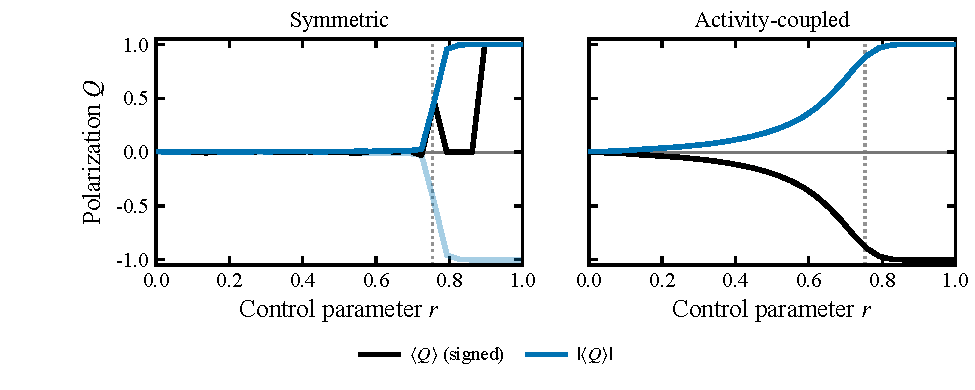
\includegraphics[width=0.92\linewidth]{s2_signed_vs_abs_q.pdf}
  \caption{Signed mean $\langle Q\rangle$ versus magnitude $|Q|$ under symmetric branch selection. In the symmetric regime, trajectories select $\pm q^\ast$ with equal probability, so $\langle Q\rangle$ cancels while $|Q|$ reveals the transition.}
  \label{fig:supp:signed-vs-abs-q}
\end{figure}

\subsection{Activity is not a passive slow variable under asymmetry}
The main text interprets activity as an observable proxy for the depletion of the moderate buffer. In activity-coupled asymmetric simulations, activity often relaxes faster than polarization, implying that $a$ cannot be treated as a passive slow variable and should be tracked jointly with $q$ when testing dynamical signatures and interpreting empirical associations.

\begin{figure}[H]
  \centering
  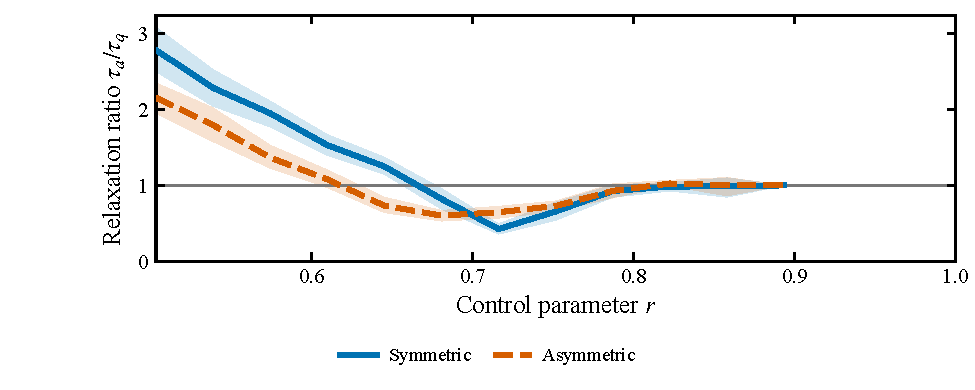
\includegraphics[width=0.92\linewidth]{s2_tau_ratio.pdf}
  \caption{Relaxation-time ratio between activity and polarization under activity-coupled asymmetry. Estimated relaxation times satisfy $\tau_a/\tau_q<1$ (baseline mean $\approx 0.70$), so activity relaxes faster than polarization.}
  \label{fig:supp:tau-ratio}
\end{figure}

\subsection{Finite-size diagnostics for locating the transition}
To estimate the transition point in finite sparse networks, we use Binder cumulant crossings because they provide a stable finite-size signature. In contrast, susceptibility peaks can shift non-monotonically with system size and can exhibit pseudo-peaks, making them less reliable for locating $r_c$ in finite simulations.

\begin{figure}[H]
  \centering
  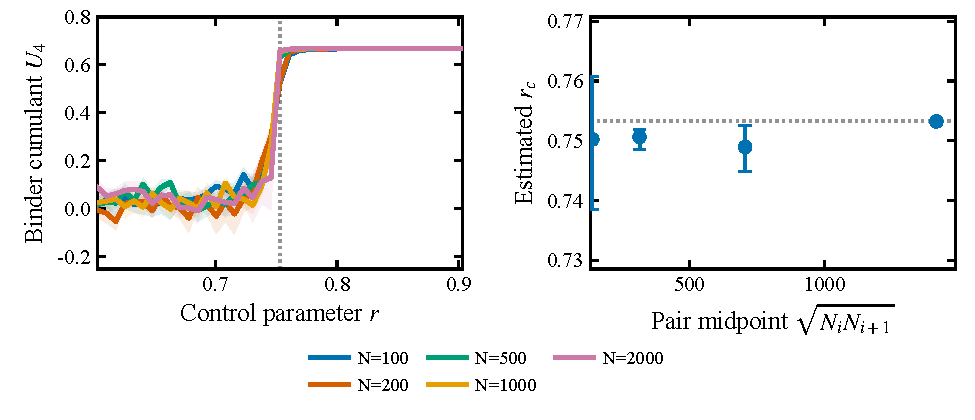
\includegraphics[width=0.92\linewidth]{s2_binder_fss.pdf}
  \caption{Finite-size scaling via Binder cumulant crossings. Curves $U_4(r;N)$ for multiple system sizes cross near the critical region, providing a stable finite-size estimator of the transition.}
  \label{fig:supp:binder-fss}
\end{figure}

\begin{figure}[H]
  \centering
  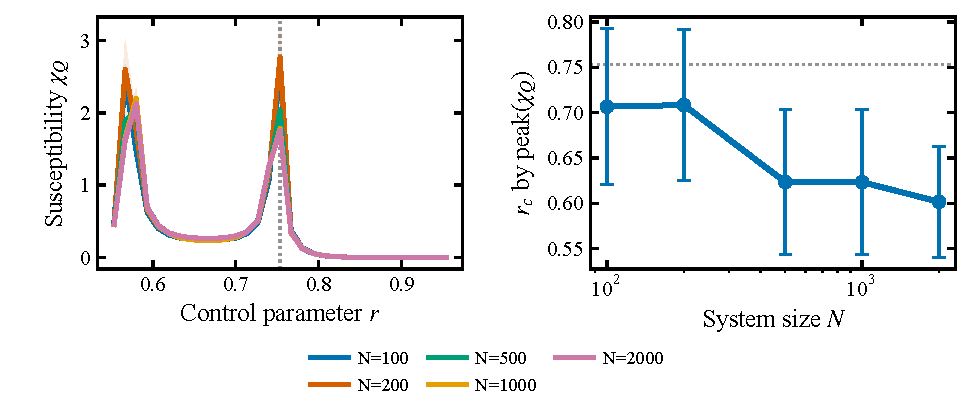
\includegraphics[width=0.92\linewidth]{s2_susceptibility_fss.pdf}
  \caption{Susceptibility peak locations across system sizes. Peaks can shift non-monotonically and exhibit finite-size artifacts compared with Binder crossings.}
  \label{fig:supp:susceptibility-fss}
\end{figure}

% -------------------------
% S4: CSD early-warning analysis
% -------------------------
\section{Early-warning signal analysis for critical slowing down}
\label{supp:s4-csd}

This section reports additional early-warning indicators for critical slowing down beyond the main-text panels.

\subsection{Early-warning statistics across the control parameter}
Approaching the critical point from below, the restoring force weakens and the dynamics become more persistent. This manifests as rising short-lag autocorrelation and variance, which are standard early-warning statistics in the critical-transition literature.

\begin{figure}[H]
  \centering
  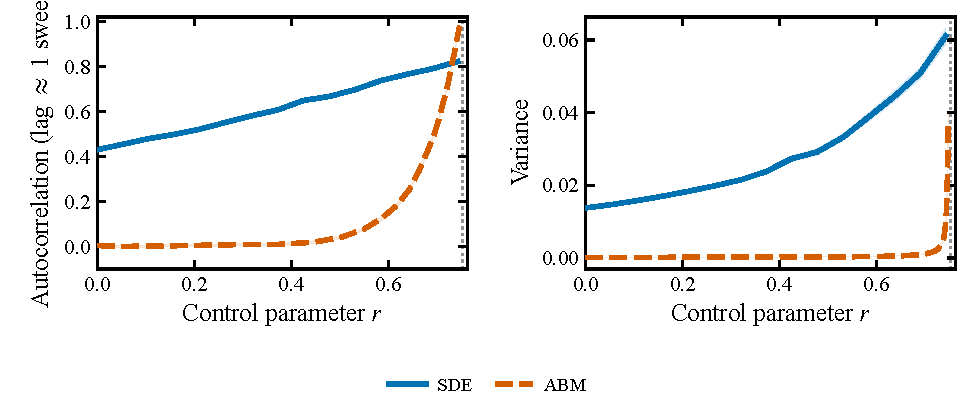
\includegraphics[width=0.92\linewidth]{s3_ews_ac_var.pdf}
  \caption{Early-warning indicators across the control parameter. Short-lag autocorrelation and variance increase as $r$ approaches $r_c$ from below.}
  \label{fig:supp:ews-ac-var}
\end{figure}

\subsection{Robustness across lag choices}
To confirm that the persistence increase is not an artifact of choosing a particular lag, we compute autocorrelation at multiple lags. The qualitative rise near criticality is consistent across lags.

\begin{figure}[H]
  \centering
  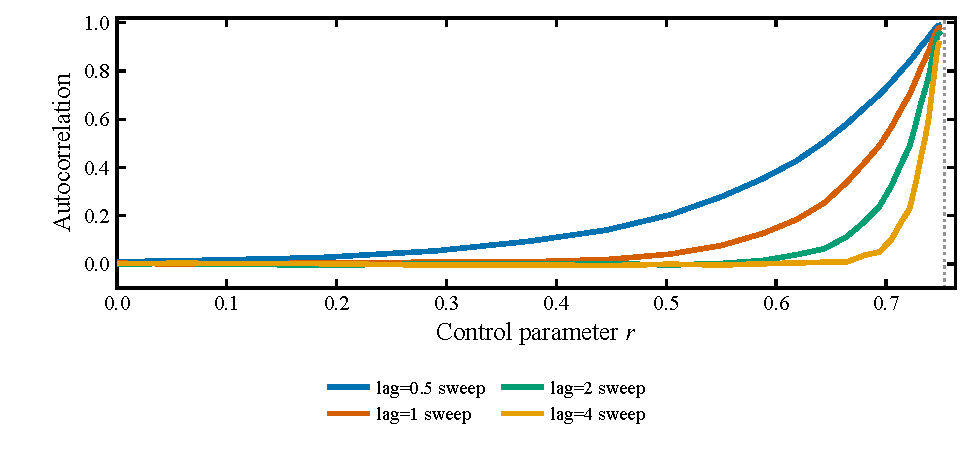
\includegraphics[width=0.92\linewidth]{s3_abm_multilag_ac.pdf}
  \caption{Multi-lag autocorrelation in ABM trajectories. Autocorrelation increases near criticality across multiple lags.}
  \label{fig:supp:abm-multilag-ac}
\end{figure}

% -------------------------
% S5: Parameter effects on the critical boundary
% -------------------------
\section{Parameter effects on the critical boundary}
\label{supp:s5-parameter}

This section provides supporting figures for the parameter-landscape results, clarifying how structural parameters move the critical boundary and documenting checks related to symmetry and finite-size effects.

\noindent\textbf{Parameter scans and estimators.} The main-text landscape figures evaluate the mean-field critical point on a dense $(\phi,\theta)$ grid over the feasible region $\theta<0.5<\phi$. Simulation-based sweeps vary information density $k\in\{10,20,50,100,200,500\}$, media ratio $n_w/n_m\in[0.1,2.0]$ (40 values), and local coupling $\beta\in\{0,0.02,0.05,0.1,0.2\}$. For each configuration we sample $r$ on a 201-point grid in $[0,1]$ and estimate $r_c$ from the maximum slope of the median $|Q|(r)$ across seeds, with 95\% confidence intervals obtained by bootstrap resampling.

\subsection{Symmetry validation}
The analytic critical point is derived in the symmetric regime. Along the symmetry constraint, the theoretical constructions satisfy neutrality conditions used in the derivation, supporting the internal consistency of the landscape map.

\begin{figure}[H]
  \centering
  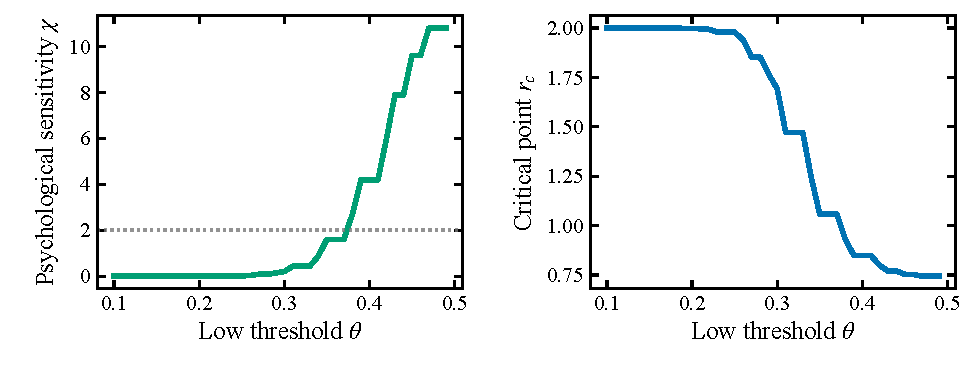
\includegraphics[width=0.92\linewidth]{s4_symmetric_diagonal.pdf}
  \caption{Symmetry diagnostics in the symmetric regime along the analytic constraint in $(\phi,\theta)$.}
  \label{fig:supp:symmetric-diagonal}
\end{figure}

\subsection{Decomposing the information-density effect}
The main text reports a non-monotonic $k$ effect on the estimated transition point. We separate this into two components: how $k$ changes the psychological sensitivity $\chi$, and how the induced $\chi(k)$ maps to $r_c(k)$.

\begin{figure}[H]
  \centering
  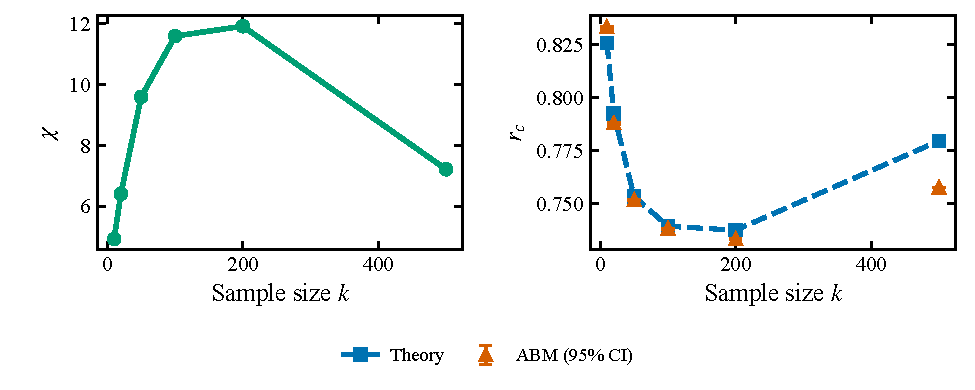
\includegraphics[width=0.92\linewidth]{s4_k_effect_split.pdf}
  \caption{Decomposing the information-density effect into sensitivity $\chi(k)$ and the induced shift in $r_c(k)$.}
  \label{fig:supp:k-effect-split}
\end{figure}

\subsection{Finite-size closure at high information density}
At very large information density ($k=500$), discrete-threshold effects and finite-size fluctuations can bias naive estimators. Local scanning and finite-size extrapolation reconcile the apparent deviation with the analytic prediction.

\begin{figure}[H]
  \centering
  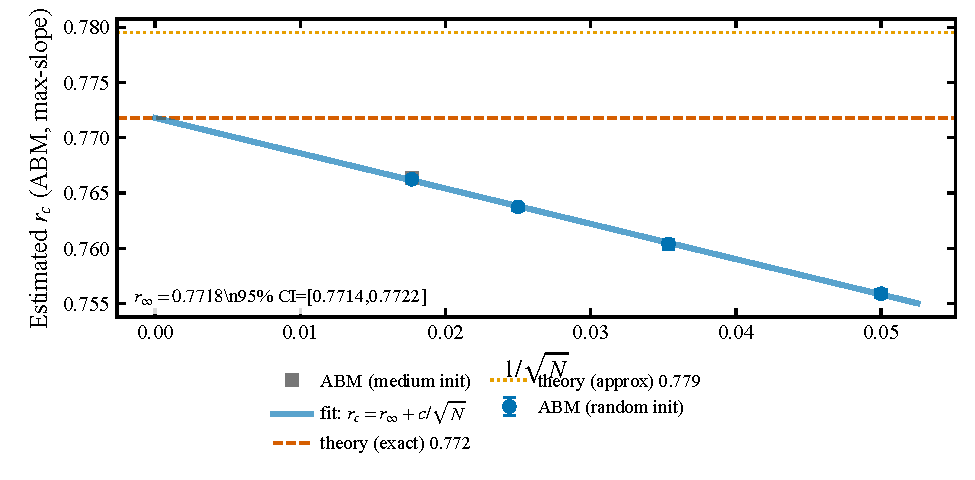
\includegraphics[width=0.92\linewidth]{s4_k500_finite_size.pdf}
  \caption{Finite-size closure for $k=500$ via local scanning and extrapolation.}
  \label{fig:supp:k500-finite-size}
\end{figure}

\subsection{Local coupling and branch-selection bias}
Beyond the well-mixed benchmark, local coupling can introduce reinforcement that both shifts the effective boundary and biases branch selection. These effects help interpret why topology and local interactions matter for proximity to criticality.

\begin{figure}[H]
  \centering
  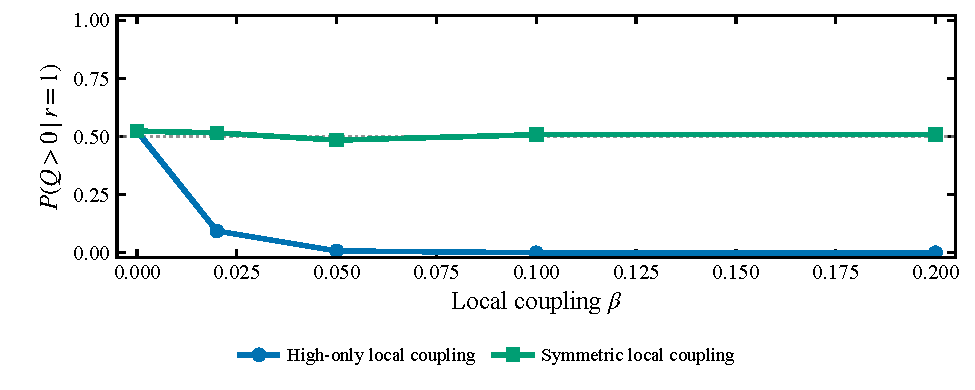
\includegraphics[width=0.92\linewidth]{s4_beta_branch_bias.pdf}
  \caption{Branch-selection bias induced by local coupling $\beta>0$.}
  \label{fig:supp:beta-branch-bias}
\end{figure}

\begin{figure}[H]
  \centering
  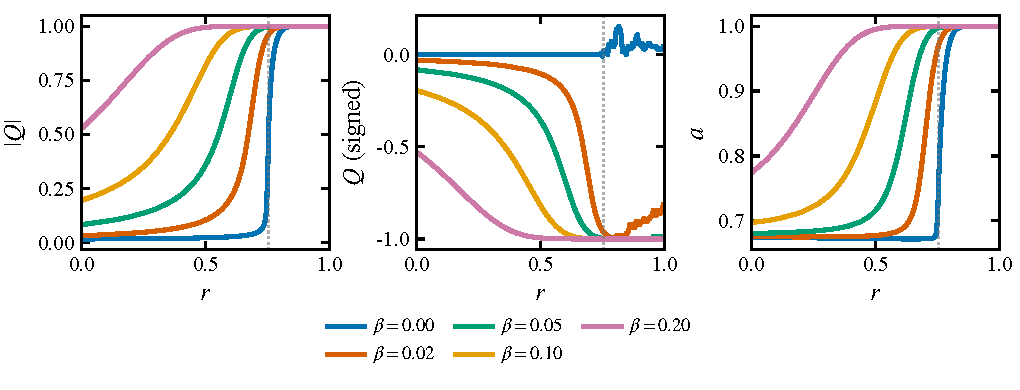
\includegraphics[width=0.92\linewidth]{s4_beta_q_a.pdf}
  \caption{Joint $(q,a)$ behavior under local coupling, showing how polarization and activity co-vary as the boundary shifts.}
  \label{fig:supp:beta-q-a}
\end{figure}

\subsection{Parameter importance and interaction}
To summarize the magnitude of boundary shifts across parameters, we compare the full scan range $\Delta r_c=\max(r_c)-\min(r_c)$ (normalized by the baseline $r_c$). We also show a theory-level interaction: higher sensitivity $\chi(k)$ amplifies the leverage of media ecology on $r_c$.

\begin{figure}[H]
  \centering
  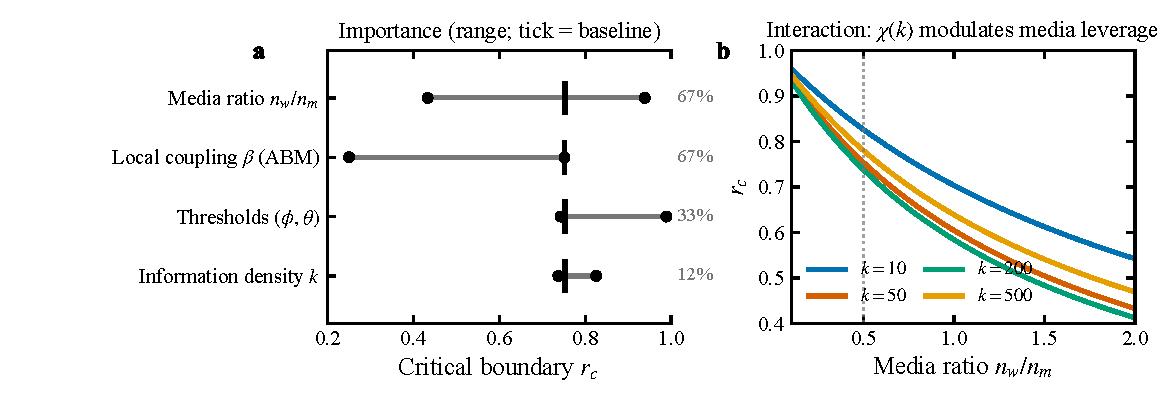
\includegraphics[width=0.92\linewidth]{fig_supp_param_importance.pdf}
  \caption{Parameter-importance summary and theory interaction. (a) Range of $r_c$ across parameter sweeps (line: min--max; tick: baseline), annotated by $\Delta r_c/r_{c,\mathrm{base}}$. (b) Theory prediction of $r_c(n_w/n_m)$ for representative $k$ values (vertical dotted line: baseline ratio).}
  \label{fig:supp:param-importance}
\end{figure}

% -------------------------
% S6: Empirical analysis details and density diagnostics
% -------------------------
\section{Empirical analysis details and density diagnostics}
\label{supp:s6-empirical}

This section provides supporting empirical figures, focusing on sampling-density constraints and on diagnostics aligned to the theoretical signatures.

\noindent\textbf{Empirical subsets.} We use the same subset naming as in the main text: the \emph{pooled dataset} (all eligible segments) and the \emph{high-density subset} (segments with sufficient within-window coverage for stable $r_{\text{proxy}}$ estimation). When shown for context only, we also report a topic-focused \emph{single-topic subset}.

\subsection{Time-series overview and segmentation rationale}
We summarize the window-level proxies used in the main text and highlight missingness patterns. This motivates segment-based aggregation and density-aware diagnostics used in subsequent panels.

\begin{figure}[H]
  \centering
  
\includegraphics[width=0.92\linewidth]{s5_time_series_overview.pdf}
  \caption{Time-series overview and sampling density. We show the 4-hour aggregates used to compute window-level proxies $(Q,a,r_{\text{proxy}})$, highlighting non-uniform sampling density and missing windows that motivate segment-based aggregation in the main-text analyses.}
  \label{fig:supp:time-series-overview}
\end{figure}

\subsection{Scatter diagnostics for the two empirical signatures}
To connect directly to the theoretical mechanism, we evaluate two segment-level associations under the primary 4-hour aggregation: elevated activity predicting larger polarization jumps, and increased user-generated dominance predicting higher polarization volatility. Density stratification is shown to diagnose coverage-driven confounds. The main text reports the density-controlled H2 estimate under 12-hour aggregation; the 4-hour diagnostics here provide additional context across datasets and missingness patterns.

\begin{figure}[H]
  \centering
  
\includegraphics[width=0.92\linewidth]{s5_scatter_h1_h2.pdf}
  \caption{Scatter diagnostics for empirical signatures under the primary 4-hour aggregation. We show segment-level associations for the activity--jump and media-dominance--volatility tests, including density-stratified views used to diagnose sampling-coverage confounds.}
  \label{fig:supp:scatter-h1-h2}
\end{figure}

\subsection{Event-aligned early-warning analysis under realistic missingness}
We additionally assess early-warning behavior by aligning autocorrelation/variance indicators to jump events. Continuity requirements can make high-frequency aggregation infeasible in sparse datasets, which limits the strength of event-aligned tests.

\begin{figure}[H]
  \centering
  
\includegraphics[width=0.92\linewidth]{s5_eventstudy_h4.pdf}
  \caption{Event-aligned early-warning diagnostics under realistic missingness. We report event-aligned trajectories for autocorrelation and variance indicators under the primary 4-hour aggregation and illustrate how higher-frequency aggregation can become infeasible due to continuity requirements.}
  \label{fig:supp:eventstudy-h4}
\end{figure}

\subsection{H2 density diagnostics: 4H versus 12H aggregation}
The media-dominance--volatility association is sensitive to sampling density and missingness. Under the primary 4-hour aggregation, the raw correlation is positive but largely attenuates after controlling for segment sampling density (number of valid windows per week). Aggregating to 12-hour windows increases per-window sample size at the cost of temporal granularity and yields more stable within-segment estimates of $r_{\text{proxy}}$ and volatility; under this aggregation, the density-controlled association remains significant.

\begin{figure}[H]
  \centering
  \begin{subfigure}[b]{0.92\linewidth}
    \centering
    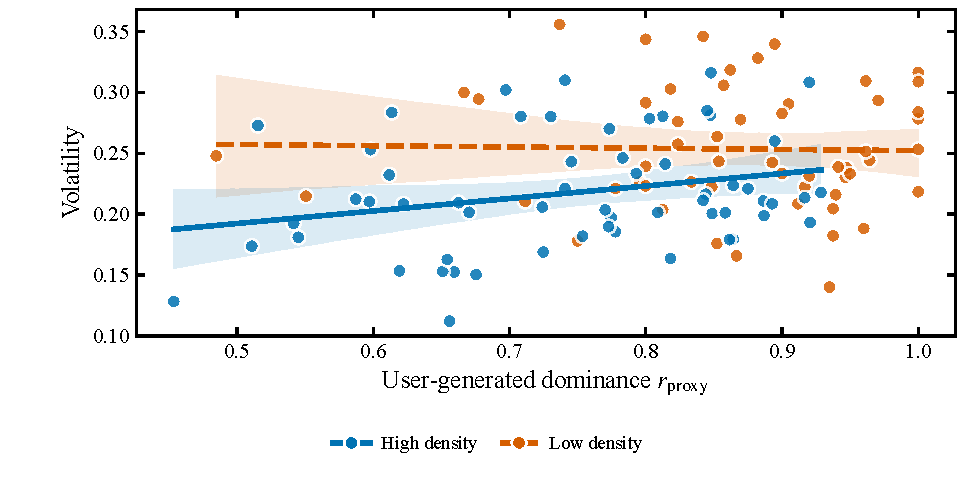
\includegraphics[width=\linewidth]{s5_h2_density_4h.pdf}
    \caption{}
  \end{subfigure}
  \vspace{0.6em}
  \begin{subfigure}[b]{0.92\linewidth}
    \centering
    
\includegraphics[width=\linewidth]{s5_h2_density_12h.pdf}
    \caption{}
  \end{subfigure}
  \caption{Density diagnostics for the media-dominance--volatility signature under two aggregation scales (high-density subset). \textbf{Top:} 4-hour aggregation (Pearson $r=0.265$, $p=0.00434$) attenuates after controlling for segment sampling density (partial $r=0.078$, $p=0.411$). \textbf{Bottom:} 12-hour aggregation yields a stronger association (Pearson $r=0.429$, $p=6.03\times 10^{-7}$) that remains significant after density control (partial $r=0.386$, $p=8.79\times 10^{-6}$). Solid/dashed lines show groupwise linear fits with 95\% bootstrap bands.}
  \label{fig:supp:h2-density-12h}
\end{figure}

% Add additional supplementary notes, figures, and tables below.

\FloatBarrier
\bibliographystyle{unsrt}
\bibliography{references}
\end{document}
